\subsection{基于 Pyside 6 的主界面}

\subsection{插件配置页面}

\subsection{托盘后台界面}

通过运行 main.py 后,托盘中会出现一个图标,当鼠标悬停于其上时,可以查看当前的登录状态,使用鼠标右键退出该插件程序。

\begin{figure}[H]
    \centering
    \begin{subfigure}[b]{0.35\textwidth}
        \centering
        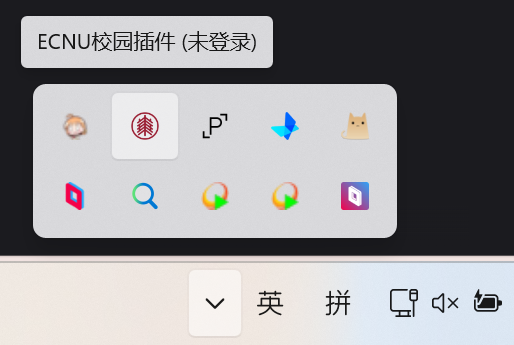
\includegraphics[width=0.8\textwidth]{img/tray_interface.png}
        \caption{处于任务栏的托盘}
        \label{fig:tray_interface}
    \end{subfigure}
    \hspace{0.06\textwidth}
    \begin{subfigure}[b]{0.3\textwidth}
        \centering
        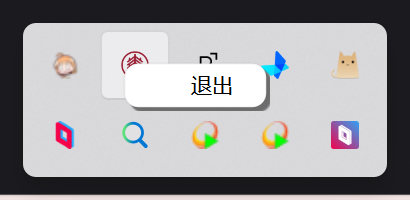
\includegraphics[width=\textwidth]{img/tray_exit.png}
        \caption{托盘退出按钮}
        \label{fig:tray_exit}
    \end{subfigure}
    \caption{托盘界面与退出按钮}
    \label{fig:tray_combined}
\end{figure}

